\section{System Design and Structure}
%
\setlength{\parindent}{0pt}
%
\subsection{CRC Cards}
% LEFT
\begin{minipage}[t]{0.49\textwidth}
    \centering
	\vspace{0pt}
    \begin{tabular}{|p{0.55\textwidth}|p{0.3\textwidth}|}
        \hline
        \rowcolor[HTML]{C0C0C0}
        \multicolumn{2}{|c|}{\cellcolor[HTML]{C0C0C0}\textbf{User}} \\ \hline
        \rowcolor[HTML]{C0C0C0}
        Responsibilities & Collaborators \\ \hline
        \begin{tabular}[c]{@{}l@{}}Name\\ ID \small{(unique, final)}\\ Address\\ Phone Number\\ \\ Show Information\\ Register Patient\end{tabular} & \begin{tabular}[c]{@{}l@{}}Patient\\ Department\end{tabular} \\ \hline
    \end{tabular}%
    %
    \bigbreak\noindent%
    %
    \begin{tabular}{|p{0.55\textwidth}|p{0.3\textwidth}|}
        \hline
        \rowcolor[HTML]{C0C0C0}
        \multicolumn{2}{|c|}{\cellcolor[HTML]{C0C0C0}\textbf{Doctor}\textit{\small{ extends User}}} \\ \hline
        \rowcolor[HTML]{C0C0C0}
        Responsibilities & Collaborators \\ \hline
        \begin{tabular}[c]{@{}l@{}}Name\\ ID \small{(unique, final)}\\ Address\\ Phone Number\\ Department\\ Speciality\\ \\ Show Information\\ Register Patient\\ Admit Patient\\ Discharge Patient\\ Assign Bed\\ Get Patients medical data\\ Edit patient medical data\end{tabular} & \begin{tabular}[c]{@{}l@{}}Department\\ Patient\\ Bed\end{tabular} \\ \hline
    \end{tabular}%
    %
    \bigbreak\noindent%
    %
    \begin{tabular}{|p{0.55\textwidth}|p{0.3\textwidth}|}
        \hline
        \rowcolor[HTML]{C0C0C0}
        \multicolumn{2}{|c|}{\cellcolor[HTML]{C0C0C0}\textbf{Department}\textit{\small{ Abstract}}} \\ \hline
        \rowcolor[HTML]{C0C0C0}
        Responsibilities & Collaborators \\ \hline
        \begin{tabular}[c]{@{}l@{}}Name\\ ID \small{(unique, final)}\\ User List\\ \\ Add User\\ Remove User\end{tabular} & \begin{tabular}[c]{@{}l@{}}User\\ Patient\end{tabular} \\ \hline
    \end{tabular}%
    %
    \bigbreak\noindent%
    %
    \begin{tabular}{|p{0.55\textwidth}|p{0.3\textwidth}|}
        \hline
        \rowcolor[HTML]{C0C0C0}
        \multicolumn{2}{|c|}{\cellcolor[HTML]{C0C0C0}\textbf{Outpatient}\textit{\small{ extends Department}}} \\ \hline
        \rowcolor[HTML]{C0C0C0}
        Responsibilities & Collaborators \\ \hline
        \begin{tabular}[c]{@{}l@{}}Name\\ ID \small{(unique, final)}\\ User List\\ Patient List\\ Capacity\\ \\ Add User\\ Remove User\\ Add Patient\\ Remove Patient\end{tabular} & \begin{tabular}[c]{@{}l@{}}User\\ Patient\end{tabular} \\ \hline
    \end{tabular}%
\end{minipage}%
% RIGHT
\begin{minipage}[t]{0.49\textwidth}
    \centering
	\vspace{0pt}
    \begin{tabular}{|p{0.55\textwidth}|p{0.3\textwidth}|}
        \hline
        \rowcolor[HTML]{C0C0C0}
        \multicolumn{2}{|c|}{\cellcolor[HTML]{C0C0C0}\textbf{Nurse}\textit{\small{ extends User}}} \\ \hline
        \rowcolor[HTML]{C0C0C0}
        Responsibilities & Collaborators \\ \hline
        \begin{tabular}[c]{@{}l@{}}Name\\ ID \small{(unique, final)}\\ Address\\ Phone Number\\ Department\\ \\ Show Information\\ Register Patient\\ Admit Patient\\ Discharge Patient\\ Assign Bed\\ Get Patients medical data\\ Edit patient medical data\end{tabular} & \begin{tabular}[c]{@{}l@{}}Department\\ Patient\\ Bed\end{tabular} \\ \hline
    \end{tabular}%
    %
    \bigbreak\noindent%
    %
    \begin{tabular}{|p{0.55\textwidth}|p{0.3\textwidth}|}
        \hline
        \rowcolor[HTML]{C0C0C0}
        \multicolumn{2}{|c|}{\cellcolor[HTML]{C0C0C0}\textbf{Admin}\textit{\small{ extends User}}} \\ \hline
        \rowcolor[HTML]{C0C0C0}
        Responsibilities & Collaborators \\ \hline
        \begin{tabular}[c]{@{}l@{}}Name\\ ID \small{(unique, final)}\\ Address\\ Phone Number\\ Department\\ \\ Show Information\\ Register Patient\\ Admit Patient\\ Discharge Patient\\ Assign Bed\\ Add User\\ Remove User\\ Get Patients medical data\\ Edit patient medical data\end{tabular} & \begin{tabular}[c]{@{}l@{}}Department\\ Patient\\ Bed\\ User\\ Nurse\\ Doctor\end{tabular} \\ \hline
    \end{tabular}%
    %
    \bigbreak\noindent%
    %
    \begin{tabular}{|p{0.55\textwidth}|p{0.3\textwidth}|}
        \hline
        \rowcolor[HTML]{C0C0C0}
        \multicolumn{2}{|c|}{\cellcolor[HTML]{C0C0C0}\textbf{Inpatient}\textit{\small{ extends Department}}} \\ \hline
        \rowcolor[HTML]{C0C0C0}
        Responsibilities & Collaborators \\ \hline
        \begin{tabular}[c]{@{}l@{}}Name\\ ID \small{(unique, final)}\\ User List\\ Patient List\\ Bed List\\ Next Bed Index\\ Capacity\\ \\ Add User\\ Remove User\\ Add Patient\\ Remove Patient\end{tabular} & \begin{tabular}[c]{@{}l@{}}User\\ Patient\\ Bed\end{tabular} \\ \hline
    \end{tabular}%
\end{minipage}%

% LEFT
\begin{minipage}[t]{0.49\textwidth}
    \centering
	\vspace{0pt}
    \begin{tabular}{|p{0.55\textwidth}|p{0.3\textwidth}|}
        \hline
        \rowcolor[HTML]{C0C0C0}
        \multicolumn{2}{|c|}{\cellcolor[HTML]{C0C0C0}\textbf{Management}\textit{\small{ extends Department}}} \\ \hline
        \rowcolor[HTML]{C0C0C0}
        Responsibilities & Collaborators \\ \hline
        \begin{tabular}[c]{@{}l@{}}Name\\ ID \small{(unique, final)}\\ User List\\ \\ Add User\\ Remove User\end{tabular} & \begin{tabular}[c]{@{}l@{}}User\\ Patient\end{tabular} \\ \hline
    \end{tabular}%
    %
    \bigbreak\noindent%
    %
    \begin{tabular}{|p{0.55\textwidth}|p{0.3\textwidth}|}
        \hline
        \rowcolor[HTML]{C0C0C0}
        \multicolumn{2}{|c|}{\cellcolor[HTML]{C0C0C0}\textbf{Patient}} \\ \hline
        \rowcolor[HTML]{C0C0C0}
        Responsibilities & Collaborators \\ \hline
        \begin{tabular}[c]{@{}l@{}}Name\\ ID \small{(unique, final)}\\ Phone Number\\ Address\\ Deceased\\ Health Record\\ Department\end{tabular} & \begin{tabular}[c]{@{}l@{}}Department\end{tabular} \\ \hline
    \end{tabular}
\end{minipage}%
% RIGHT
\begin{minipage}[t]{0.49\textwidth}
    \centering
	\vspace{0pt}
    \begin{tabular}{|p{0.55\textwidth}|p{0.3\textwidth}|}
        \hline
        \rowcolor[HTML]{C0C0C0}
        \multicolumn{2}{|c|}{\cellcolor[HTML]{C0C0C0}\textbf{Emergency}\textit{\small{ extends Department}}} \\ \hline
        \rowcolor[HTML]{C0C0C0}
        Responsibilities & Collaborators \\ \hline
        \begin{tabular}[c]{@{}l@{}}Name\\ ID \small{(unique, final)}\\ User List\\ Patient List\\ \\ Add User\\ Remove User\\ Add Patient\\ Remove Patient\end{tabular} & \begin{tabular}[c]{@{}l@{}}User\\ Patient\end{tabular} \\ \hline
    \end{tabular}%
    %
    \bigbreak\noindent%
    %
    \begin{tabular}{|p{0.55\textwidth}|p{0.3\textwidth}|}
        \hline
        \rowcolor[HTML]{C0C0C0}
        \multicolumn{2}{|c|}{\cellcolor[HTML]{C0C0C0}\textbf{Bed}} \\ \hline
        \rowcolor[HTML]{C0C0C0}
        Responsibilities & Collaborators \\ \hline
        \begin{tabular}[c]{@{}l@{}}ID \small{(unique, final)}\\ Patient\\ Department\\ \\ Show Information\end{tabular} & \begin{tabular}[c]{@{}l@{}}Patient\\ Department\end{tabular} \\ \hline
    \end{tabular}%
\end{minipage}%
%
\subsection{UML Class Diagram}
%
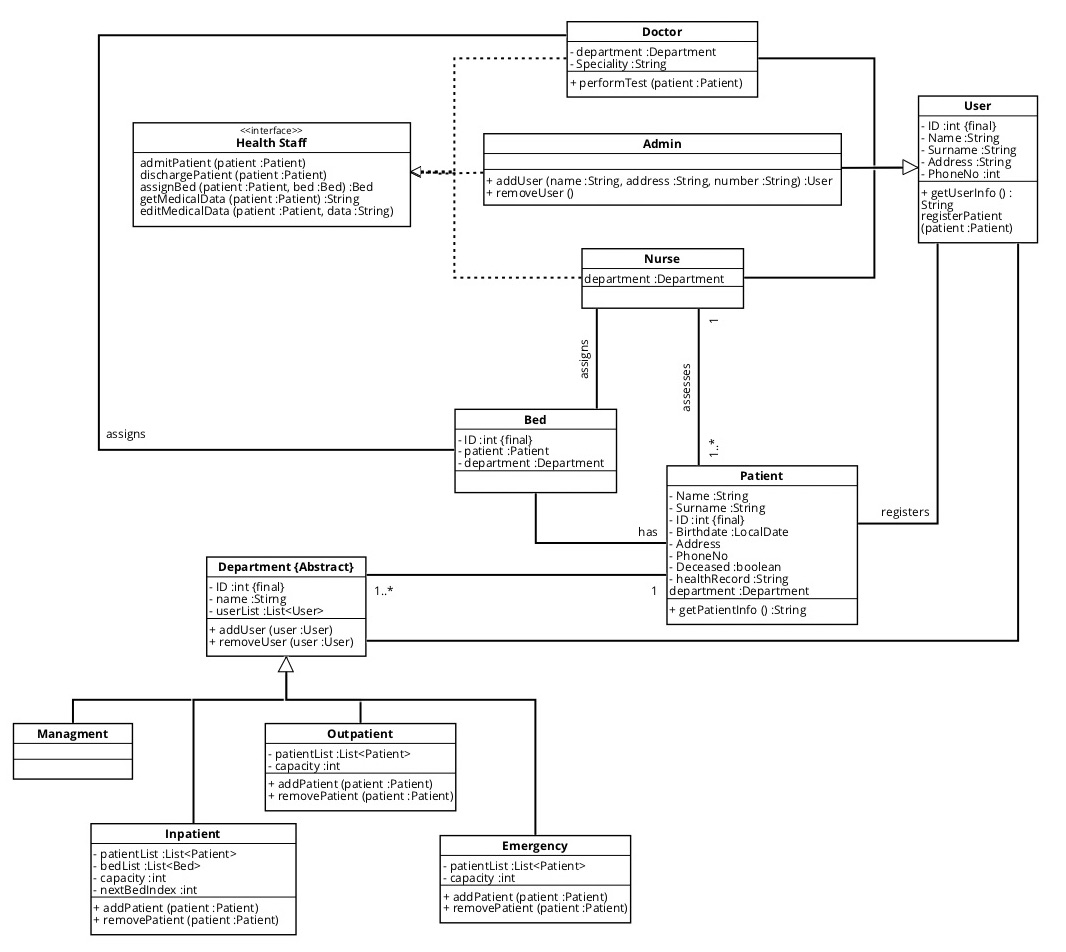
\includegraphics[width=0.9\textwidth]{Figures/ClassDiagram}
%
\subsection{User Stories}
%
\subsubsection*{M1 Patient Registration}
%
\textbf{AS A} User\hfill \break
\textbf{I WANT} To register a new patient\hfill \break
\textbf{SO THAT} I can save their basic information in the system\hfill \medbreak
%
\textbf{AS A} User\hfill \break
\textbf{I WANT} To edit a patient's information\hfill \break
\textbf{SO THAT} the system can maintain validity if a patient's information changes.\hfill \medbreak
%
\textbf{AS A} User\hfill \break
\textbf{I WANT} To search for a certain patient based on identifying information (name, birth date, patient number etc.)\hfill \break
\textbf{SO THAT} I can easily find patients in the system\hfill \medbreak
%
\subsubsection*{M2 Staff Management}
%
\textbf{AS AN} Admin\hfill \break
\textbf{I WANT} To register new staff members\hfill \break
\textbf{SO THAT} there is accurate record keeping in the system\hfill \medbreak
%
\textbf{AS AN} Admin\hfill \break
\textbf{I WANT} To view all staff member information\hfill \break
\textbf{SO THAT} I can see information about all staff in the system\hfill \medbreak
%
\textbf{AS AN} Admin\hfill \break
\textbf{I WANT} To edit staff member information\hfill \break
\textbf{SO THAT} I can maintain the validity of the system if something with a staff member changes\hfill \medbreak
%
\textbf{AS A} User\hfill \break
\textbf{I WANT} To view all staff members and their basic information (name and email only)\hfill \break
\textbf{SO THAT} I can communicate with my colleagues\hfill \medbreak
%
\textbf{AS A} User\hfill \break
\textbf{I WANT} To be able to search for staff members by their name or email\hfill \break
\textbf{SO THAT} I can access the rest of their basic information (name/email)\hfill \medbreak
%
\textbf{AS AN} Admin\hfill \break
\textbf{I WANT} To search for all users with a specific criteria (name, email, birth date, department, job title etc.)\hfill \break
\textbf{SO THAT} I can see all staff members who fulfil the criteria\hfill \medbreak
%
\subsubsection*{M3 Health Facility Management}
%
\textbf{AS A} User\hfill \break
\textbf{I WANT} To See how many beds are available in a department\hfill \break
\textbf {SO THAT} I can check if a department is at capacity\hfill \medbreak
%
\textbf{AS A} User\hfill \break
\textbf{I WANT} To be classified by a specific department\hfill \break
\textbf {SO THAT} I can have one department in which I work\hfill \medbreak
%
\textbf{AS A} User\hfill \break
\textbf{I WANT} To see a list of the departments in the hospital\hfill \break
\textbf {SO THAT} See what my options are for admitting a patient\hfill \medbreak
%
\subsubsection*{M4 Patient Admission}
%
\textbf {AS A} User\hfill \break
\textbf{I WANT} To register a new patient by entering their non-medical data\hfill \break
\textbf {SO THAT} I admit new patients\hfill \medbreak
%
\textbf{AS A} Nurse\hfill \break
\textbf{I WANT} To allocate a patient to a bed (inpatient)\hfill \break
\textbf{SO THAT} The patient is admitted to the department and can receive care.\hfill \medbreak
%
\textbf{AS A} Doctor\hfill \break
\textbf{I WANT} To call on a patient (outpatient)\hfill \break
\textbf{SO THAT} The patient can occupy a bed and receive care.\hfill \break
%
\textbf{AS A} Nurse\hfill \break
\textbf{I WANT} To discharge a patient\hfill \break
\textbf{SO THAT} The patient is no longer occupying a bed when treatment is done.\hfill \medbreak
%
\textbf{AS A} Nurse\hfill \break
\textbf{I WANT} To Move a patient to a new department\hfill \break
\textbf{SO THAT} The patient is discharged from one department and admitted to another.\hfill \medbreak
%
\textbf{AS A} Nurse\hfill \break
\textbf{I WANT} To move a patient within the current department\hfill \break
\textbf{SO THAT} The patient can be moved to another bed as needed.\hfill \medbreak
%
\subsubsection*{M5 User Interface}
%
\textbf{AS A} User\hfill \break
\textbf{I WANT} To log in\hfill \break
\textbf{SO THAT} I can access the HMS\hfill \medbreak
%
\textbf{AS A} User\hfill \break
\textbf{I WANT} To interface with the HMS\hfill \break
\textbf{SO THAT} I can manipulate or access patient and staff information\hfill \medbreak
%
\subsubsection*{O2 User Management}
%
\textbf{AS A} User\hfill \break
\textbf{I WANT} To have access to the functionality appropriate for my job \hfill \break
\textbf{SO THAT} i can do my job\hfill \medbreak
%
\subsubsection*{O4 Persistency Layer}
%
\textbf{AS A} User\hfill \break
\textbf{I WANT} To open and close the system without losing data\hfill \break
\textbf{SO THAT} I can still access patient and staff information\hfill \medbreak
%
\textbf{AS A} User\hfill \break
\textbf{I WANT} To move a patient into my department by admitting them\hfill \break
\textbf{SO THAT} I can access their previous health data that is saved in the system\hfill \medbreak
%
\subsubsection*{O6 Advanced Query Mechanism}
%
\textbf{AS A} User\hfill \break
\textbf{I WANT} To I want to be able so view simple statistics describing departments and the hospital in general\hfill \break
\textbf{SO THAT} I can get an overview of the status\hfill \medbreak
%
\subsubsection*{Miscellaneous User Stories}
%
\textbf{AS A} User\hfill \break
\textbf{I WANT} To read a patients non-Medical data\hfill \break
\textbf{SO THAT} I can see non medical data\hfill \medbreak
%
\textbf{AS A} Nurse\hfill \break
\textbf{I WANT} To read a patients medical data in my department\hfill \break
\textbf{SO THAT} I can see the medical data of all patients in my department\hfill \medbreak
%
\textbf{AS A} Nurse\hfill \break
\textbf{I WANT} To edit a patients medical data\hfill \break
\textbf{SO THAT} I can edit the Medical data of all patients in my department\hfill \medbreak
%
\newpage
%
Access level works as shown in the following hierarchy:\hfill \break
$User < Nurse < Doctor < Admin$\hfill \bigbreak
%
Nurses, Doctors, and Admin can do anything users have access to and so on...\hfill \bigbreak
%
\textbf{Users:}
\begin{itemize}
    \item User
    \item Nurse
    \item Doctor
    \item Admin
\end{itemize}

\textbf{Departments:}
\begin{itemize}
    \item Inpatients
    \item outpatients
    \item Emergency
    \item ??
\end{itemize}
%
\medbreak
%
\begin{table}[h!]
    \begin{tabular}{ll}
        \textbf{Medical Data} & \textbf{Non-Medical Data} \\
        Health Record         & Name                      \\
        Alive?                & Surname                   \\
        Height                & Address                   \\
        Weight                & Phone                     \\
        Perscriptions         & ID number                 \\
        Age                   & Department                \\
        Blood Type            &                          
    \end{tabular}
\end{table}